\documentclass[a4paper,10pt,ngerman]{scrartcl}
\usepackage{babel}
\usepackage[T1]{fontenc}
\usepackage[utf8x]{inputenc}
\usepackage[a4paper,margin=2.5cm,footskip=0.5cm]{geometry}
\usepackage{listings}

\newcommand{\Aufgabe}{Aufgabe 2: Simultane Labyrinthe} 
\newcommand{\TeilnahmeId}{74130}                
\newcommand{\Name}{Matthew Greiner}           

\usepackage{scrlayer-scrpage, lastpage}
\setkomafont{pageheadfoot}{\large\textrm}
\lohead{\Name}
\chead{\Aufgabe}
\rohead{Teilnahme-ID: \TeilnahmeId}
\cfoot*{\thepage{}/\pageref{LastPage}}

\usepackage{titling}
\setlength{\droptitle}{-1.0cm}

\lstset{ %
  language=Java,
  basicstyle=\ttfamily\small,
  keywordstyle=\color{blue},
  commentstyle=\color{green!50!black},
  stringstyle=\color{orange},
  numbers=left,
  numberstyle=\tiny\color{gray},
  stepnumber=1,
  numbersep=5pt,
  backgroundcolor=\color{white},
  showspaces=false,
  showstringspaces=false,
  tabsize=2,
  breaklines=true,
  breakatwhitespace=true,
  frame=single,
  captionpos=b,
}

\usepackage{amsmath}
\usepackage{subcaption}
\usepackage{amssymb}

\usepackage{graphicx}

\usepackage{algpseudocode}

\usepackage{listings}
\usepackage{color}
\definecolor{mygreen}{rgb}{0,0.6,0}
\definecolor{mygray}{rgb}{0.5,0.5,0.5}
\definecolor{mymauve}{rgb}{0.58,0,0.82}
\lstset{
  keywordstyle=\color{blue},commentstyle=\color{mygreen},
  stringstyle=\color{mymauve},rulecolor=\color{black},
  basicstyle=\footnotesize\ttfamily,numberstyle=\tiny\color{mygray},
  captionpos=b,
  keepspaces=true, 
  numbers=left, numbersep=5pt, showspaces=false,showstringspaces=true,
  showtabs=false, stepnumber=2, tabsize=2, title=\lstname
}
\lstdefinelanguage{JavaScript}{ 
  keywords={break, case, catch, continue, debugger, default, delete, do, else, finally, for, function, if, in, instanceof, new, return, switch, this, throw, try, typeof, var, void, while, with},
  morecomment=[l]{//},
  morecomment=[s]{/*}{*/},
  morestring=[b]',
  morestring=[b]",
  sensitive=true
}

\usepackage{cleveref}

\title{\textbf{\Huge\Aufgabe}}
\author{\LARGE Teilnahme-ID: \LARGE \TeilnahmeId \\\\
	    \LARGE Bearbeiter/-in dieser Aufgabe: \\ 
	    \LARGE \Name\\\\}
\date{\LARGE\today}

\begin{document}

\maketitle
\tableofcontents

\vspace{0.5cm}

\section{Lösungsidee}
Die Grundidee dieser Aufgabe ist es, eine möglichst kurze Anweisungssequenz zu bestimmen, mit der zwei Personen gleichzeitig von ihrem jeweiligen Startpunkt $(0,0)$ zum Zielpunkt $(n-1,m-1)$ in zwei unterschiedlichen Labyrinthen gelangen. Beide Labyrinthe haben die gleiche Grundgröße $(n$×$m)$, unter\-scheiden sich jedoch in ihrer Struktur (Platzierung der Wände). Die Herausforderung dieses Problems liegt in der Synchronisation, denn beide Personen müssen dieselbe Anweisungssequenz befolgen. Das bedeutet, dass optimale Pfade für die beiden Spieler nicht ausreichen, da eine separate Betrachtung normalerweise zu einer insgesamt längeren Abfolge von Anweisungen führen würde. Daher ist es notwendig, die beiden Labyrinthe in einem kombinierten System zu betrachten, um eine für beide gültige und gleichzeitig global minimale Sequenz zu finden. Die Teilaufgabe B wird auch direkt mit betrachtet, da bei dieser nur spezielle Felder, Gruben, hinzugefügt werden. Die Lösungsidee und Umsetzung des Algorithmus, der die Gruben betrachtet, kann auch die Labyrinthe ohne Gruben (Teilaufgabe A) lösen. 
\newline
\indent \indent Um dieses Problem zu lösen, wird es in ein Kürzeste-Wege-Problem überführt. Dazu wird ein Zustandsgraph modelliert, der alle möglichen gültigen Positionen der beiden Spieler zu jedem Zeitpunkt enthält. Ein Zustand $S$ im Graph wird dabei definiert als ein Tupel $(x_1, y_1, x_2, y_2)$, wobei $(x_1, y_1)$ die Koordinaten von Spieler 1 und $(x_2, y_2)$ die Koordinaten von Spieler 2 in ihrem Labyrinth darstellt. In diesem Graph repräsentiert eine Kante die Anwendung einer einzelnen Richtungsanweisung (←, →, ↑, ↓). Wenn eine dieser Anweisung für einen Spieler gegen eine Wand führt, bleibt der Spieler laut der Aufgabenstellung auf seiner aktuellen Position stehen. In der wird auch definiert, dass ein Spieler auf seinem Zielfeld bleibt und weitere Bewegungsanweisungen ignoriert, sobald er es erreicht hat. Außerdem wird ein Spieler auf sein Startfeld $(0,0)$ zurückgesetzt, wenn er auf eine Grube trifft. 
\\\newline
Das Ziel dieser Modellierung ist, den kürzesten Pfad im Zustandsgraphen vom Startzustand $(0, 0, 0, 0)$ zum Zielzustand $(n-1, m-1, n-1, m-1)$ zu finden. Für diese Suche bietet sich die Breadth-First-Search Methode (BFS) an, da sie garantiert den kürzesten Weg in einem ungewichteten Graphen (alle Bewegungen kosten gleich viel) findet. Allerdings ist der A-Star Suchalgorithmus auch passend, der theoretisch das Ergebnis schneller finden sollte, da bei der Suche eine Heuristik verwendet wird. Im Folgenden werden beide dieser Algorithmen umgesetzt:

\subsection{Breitensuche (BFS)}
Die Breitensuche (BFS) ist ein Graphsuchalgorithmus, der systematisch den Graph erkundet. Hier also die möglichen Bewegungen in den Labyrinthen. Sie beginnt beim Startzustand und untersucht alle erreichbaren Nachbarzustände. Anschließend werden für jeden dieser Nachbarn deren unbesuchte Nachbarn untersucht, und so weiter. Dieses Vorgehen erfolgt "Schicht für Schicht", basierend auf der Anzahl der Schritte (Kanten) vom Startzustand. Eine FIFO-Warteschlange (Queue) verwaltet die Reihenfolge der zu besuchenden Zustände. Da BFS die Zustände in der Reihenfolge ihrer Entfernung vom Start bearbeitet, findet sie garantiert den Pfad mit der geringsten Anzahl an Schritten, wenn solch ein Pfad existieren sollte. Um Endlosschleifen (u.a. aufgrund der Gruben) und Zyklen bei der Suche im Graphen zu verhindern, muss gespeichert werden, welche Zustände bereits besucht wurden. Bevor ein neuer Zustand zur Queue hinzugefügt wird, wird geprüft, ob dieser spezifische Zustand bereits besucht wurde. Wenn dies der Fall ist, wird dieser Zustand ignoriert und nicht erneut zur Queue hinzugefügt. 
\\\indent \indent Die Einführung von Gruben stellt auf den ersten Blick eine Herausforderung dar, da sie Zyklen im Pfad von einem Spieler erzeugen. Für BFS ist dies allerdings kein Problem, da sie den kombinierten Zustand $(x_1, y_1, x_2, y_2)$ betrachtet. Wenn ein Spieler in eine Grube fällt, ändert sich der kombinierte Zustand (z.B. zu $(0, 0, x_2, y_2)$). Sollte BFS durch weitere Züge (evtl. nach öfterem Fallen in Gruben) später wieder denselben Zustand erreichen, wäre dies kein Problem, da gespeichert wurde, dass dieser Zustand schon erreicht wurde. 
\subsection{A*}
Als Alternative zur Breitensuche kann auch der A* Algorithmus verwendet werden, um den kürzesten Pfad im Zustandsgraphen zu finden. A* ist ein informierter Suchalgorithmus, der zusätzlich zu den bereits zurückgelegen Kosten $(g(n))$, eine Schätzung der verbleibenden Kosten bis zum Ziel ($h(n)$, die Heuristik) berücksichtigt, um potenziell weniger Zustände durchsuchen zu müssen, um die Lösung zu finden.  
\newline
Es wird eine PriorityQueue verwendet, um zu entscheiden, welcher Zustand als nächste besucht wird. Sei 
\begin{itemize}
  \item $g(n)$ die tatsächlichen Kosten (Anzahl der Schritte/Kanten/Anweisungen) vom Startzustand bis zum Zustand $n$. 
  \item $h(n)$ eine heuristische Schätzung der minimalen Kosten (minimale Anzahl weiterer Schritte), um von Zustand $n$ zum Zielzustand zu gelangen. Diese Heuristik muss \textit{zulässig} (admissible) sein, d.h. um zu garantieren, dass die Lösung optimal ist, darf sie die tatsächlichen Kosten zum Ziel nie überschätzen.  
\end{itemize}
Dann ist die Priorität eines Zustand $n$ ist durch die Funktion 
\begin{equation}
  f(n) = g(n) + h(n) 
  \label{1}
\end{equation}
bestimmt. $f(n)$ sind die geschätzten Gesamtkosten des Pfades vom Start zum Ziel über den Zustand $n$. Mit Hilfe der PriorityQueue wählt A* immer den Zustand mit dem niedrigsten $f(n)$-Wert zur Expansion aus.  
Für diese Aufgabe, wird eine Heuristik benötigt, die die Distanz beider Spieler berücksichtigt. Eine geeignete zulässige Heuristik ist das Maximum der Manhatten-Distanzen der beiden Spieler zu ihren Zielen:
\begin{equation}
  h(n) = max( |x_1 - \text{zielX}| + |y_1 - \text{zielY}|, |x_2 - \text{zielX}| + |y_2 - \text{zielY}| ) 
  \label{2}
\end{equation}
Die Manhatten-Distanz ist die minimale Anzahl von Schritten in einem Gitter ohne Berücksichtigung von Wänden oder Gruben. Da die gemeinsame Anweisungssequenz mindestens so lang sein muss wie der (theoretisch) kürsteste Weg des Spielers, der am weitesten entfernt ist, überschätzt diese Heuristik nie die tatsächliche Anzahl der noch benötigen Schritte und ist daher zulässig.

\section{Umsetzung}
\subsection{Breitensuche (BFS)}
Bevor der Algorithmus angewendet werden kann, müssen die Labyrinthe aus den gegebenen Textdateien gelesen werden und in einer passenden Datenstruktur gespeichert werden. Die folgende Implementierung verwendet für das Speichern eines Labyrinths eine \textit{Maze}-Klasse, die das Labyrinth intern in einem \textit{byte[][]}-Array speichert. In den Eingabebeispielen der BwInf-Webseite werden die Labyrinthe der Größe $(n$×$m)$ so dargestellt, dass sich die Spieler auf Koordinaten im Bereich von $(0,0)$ bis $(n-1, m-1)$ befinden können. Es wird gegeben, zwischen welchen Koordinaten sich Wände befinden. Um in der Implementierung die begehbaren Felder und auch die Wände zwischen den Feldern explizit darzustellen, wird die Dimension des Arrays verdoppelt und um eins erhöht. Ein Labyrinth der Größe $(n$×$m)$ wird also in einem Array der Größe $(height \cdot 2 + 1)$×$(width \cdot 2 + 1)$ repräsentiert, wobei $width = n$ und $height = m$. Daraus folgt: 
\begin{itemize}
  \item Logische Felder $(x,y)$ (mit $0 \le x < width$, $0 \le y < height$) haben den Index $(x \cdot 2 + 1, y \cdot 2 + 1)$ im Array 
  \item Wände oder Freiräume zwischen den logischen Feldern haben gerade Indizes. Beispielsweise befindet sich die potenzielle vertikale Wand rechts vom Feld $(x, y)$ bei $(x \cdot 2 + 2, y \cdot 2 + 1)$ und die potenzielle horizontale Wand unterhalb von $(x, y)$ bei $(x \cdot 2 + 1, y \cdot 2 + 2)$ 
\end{itemize}
Der Wert 1 im Array markiert eine Wand, 0 einen freien Weg, und 2 eine Grube. Somit kann das Labyrinth leicht visuell dargestellt werden. Beispielsweise sehen die Labyrinthe aus der Beispieleingabe \textit{labyrinthe2.txt} wie folgt aus: 
\begin{figure}[h!]
    \centering
    \begin{subfigure}{0.45\textwidth}
        \centering
        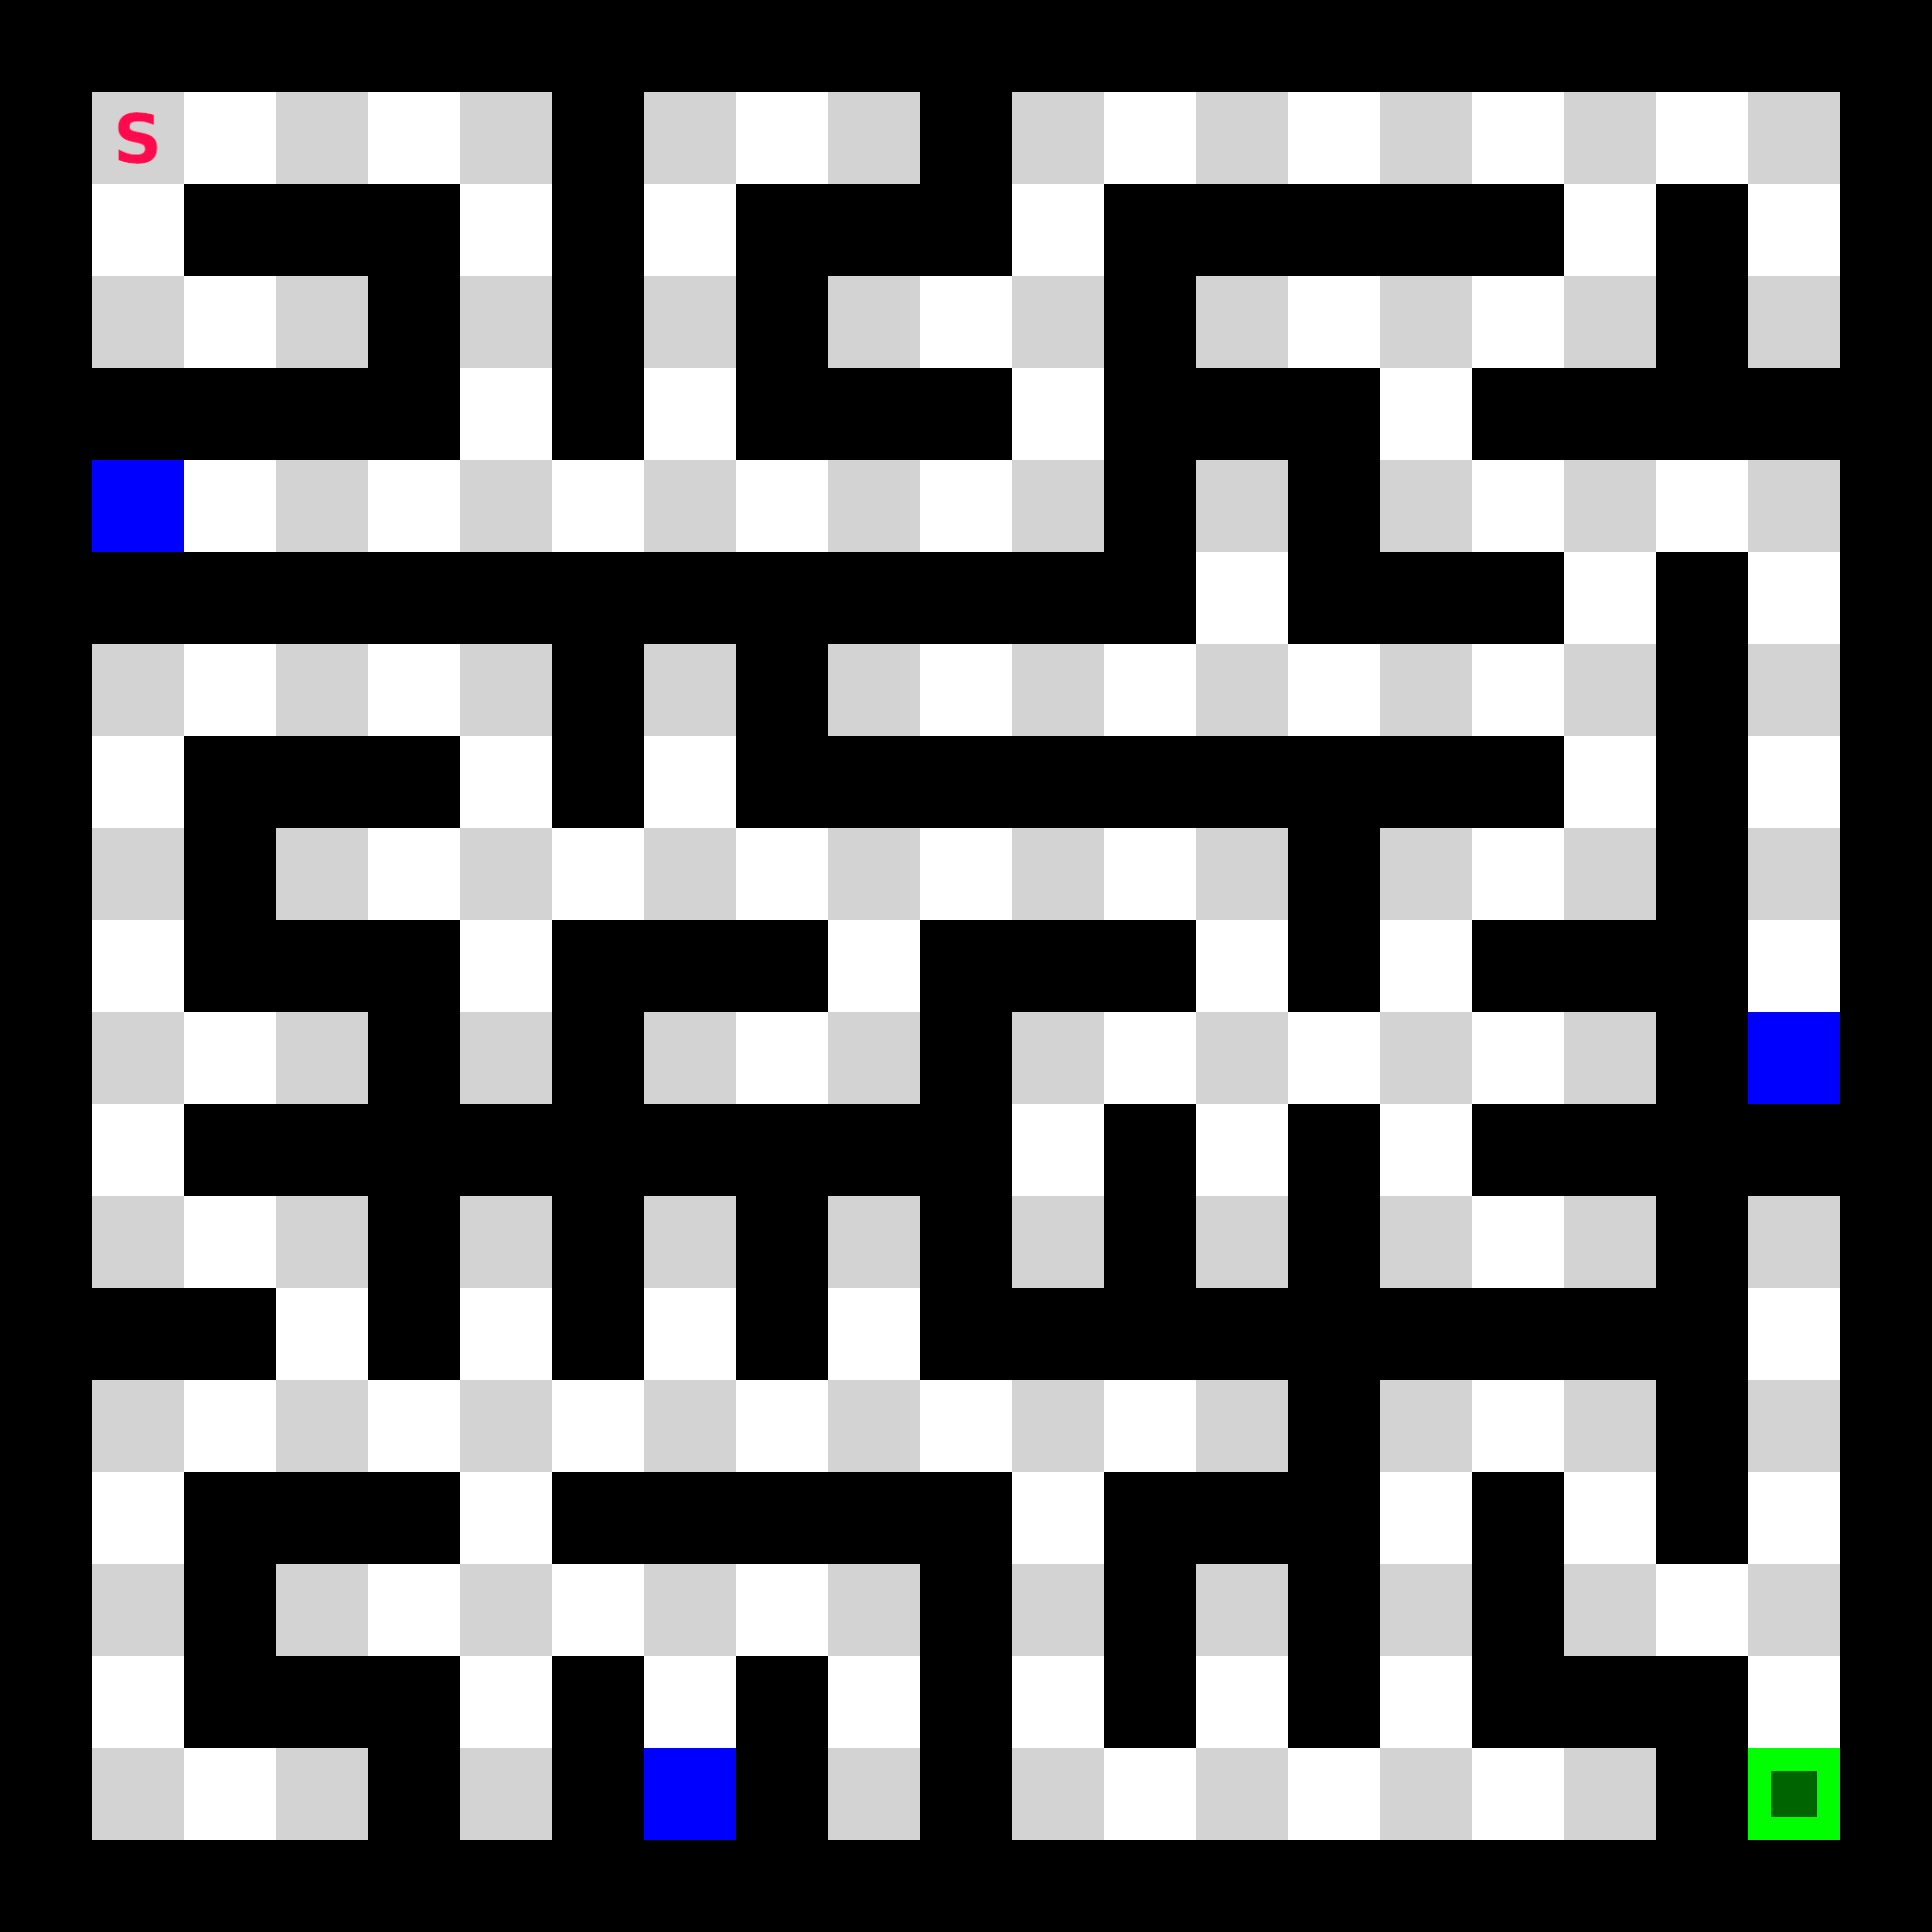
\includegraphics[width=\textwidth]{maze1.png} 
        \caption{Labyrinth für Spieler 1}
        \label{fig:bild1}
    \end{subfigure}
    \hfill
    \begin{subfigure}{0.45\textwidth}
        \centering
        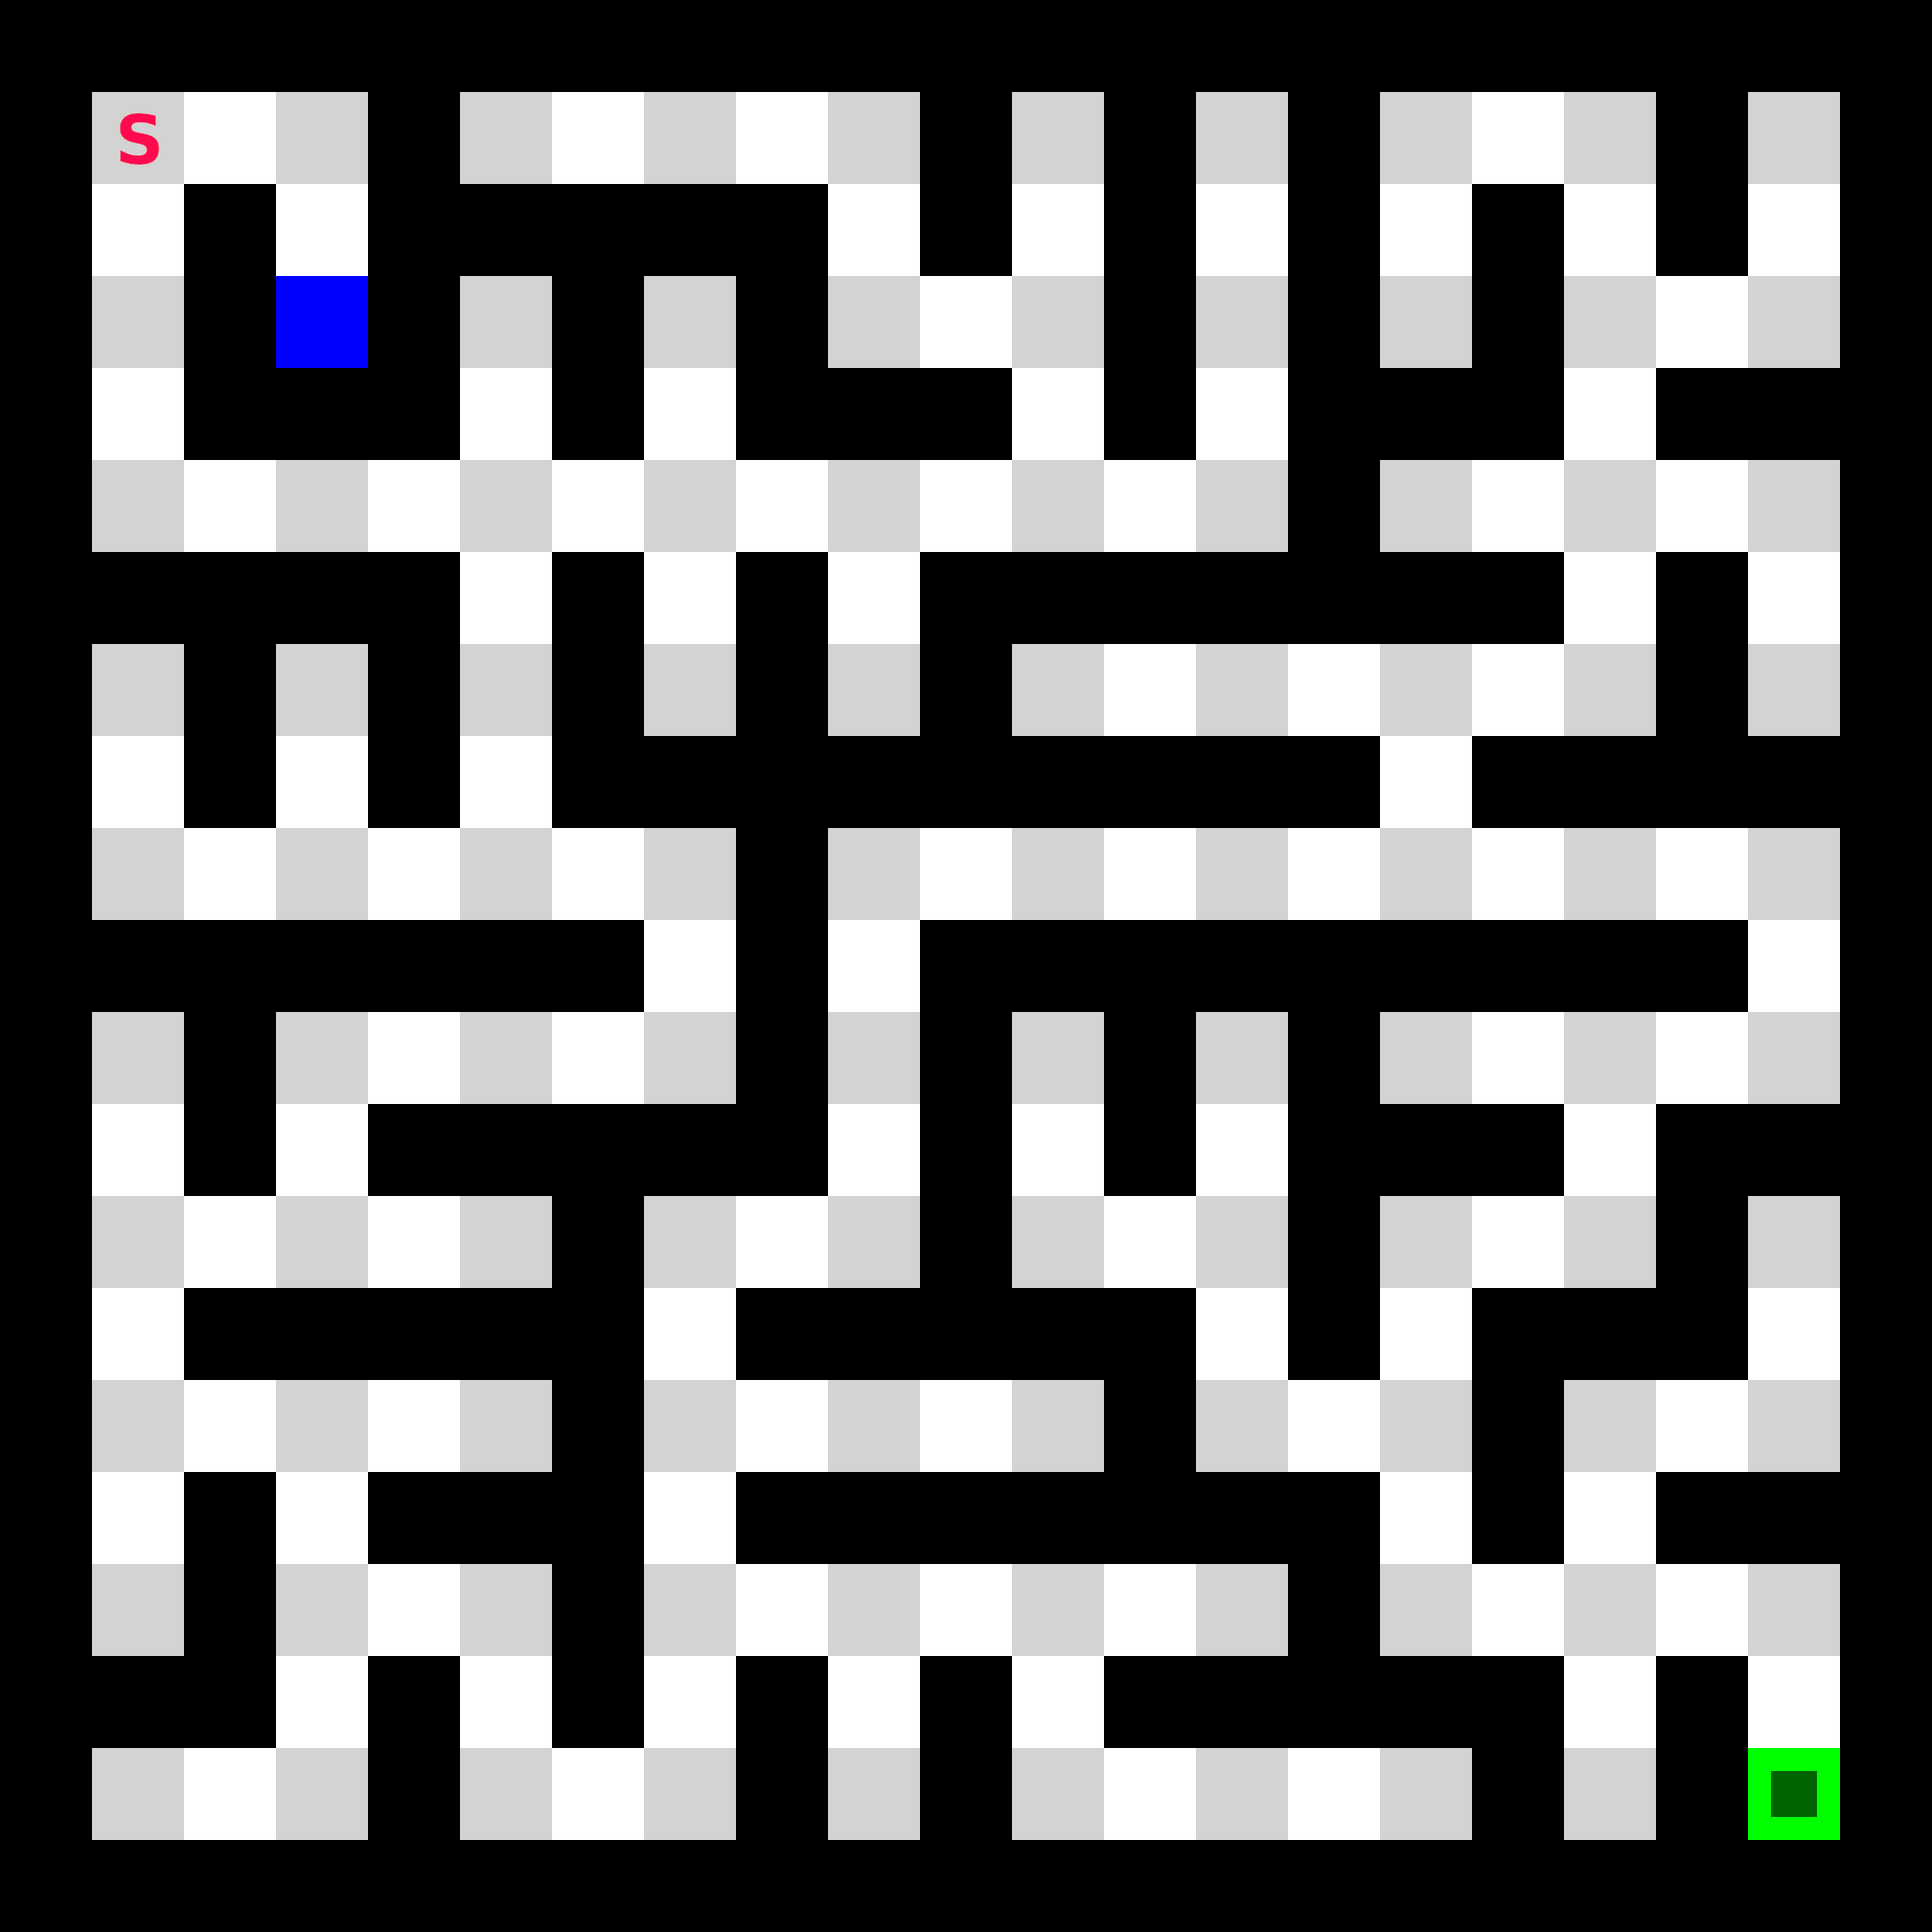
\includegraphics[width=\textwidth]{maze2.png}
        \caption{Labyrinth für Spieler 2}
        \label{fig:bild2}
    \end{subfigure}
    \caption{\textbf{Schwarz}: Wand (1 im Array), \textbf{grau}: valides logisches Feld (0 im Array), \textbf{weiß}: Freiraum zwischen zwei logischen Feldern (kann nicht betreten werden), \textbf{grün}: Zielfeld, \textbf{rotes S}: Startfeld}
    \label{fig:gesamt}
\end{figure}

Um diesen Algorithmus umzusetzen und somit die Aufgabe zu lösen, wird wie folgt vorgegangen (die Nummerierung entspricht auch der Nummerierung im Quellcode): 
\begin{enumerate}
  \item \textbf{Einlesen der Labyrinthe und deren Modellierung}\\
  Zur Einlesung der gegebenen Labyrinthe wird die Datei an den einzelnen Zeilen aufgespaltet. Die erste Zeile wird gelesen, um die logischen Dimensionen (\textit{width, height}) der Labyrinthe zu bekommen. Basierend darauf werden zwei \textit{Maze}-Objekte erstellt. 
  \\
  Zunächst werden \textit{height} Zeilen gelesen, die die Position der vertikalen Wände definieren. Der Wert $1$ an der $x$-ten Position einer Zeile markiert eine Wand rechts vom logischen Feld $(x, y)$, was intern an der Array-Position $(x\cdot2+2, y\cdot2+1)$ gespeichert wird.
  \\
  Anschließend folgen $height - 1$ Zeilen, die die horizontalen Wände beschreiben. Eine 1 an der $x$-ten Position stellt eine Wand unterhalb des logischen Feldes $(x, y)$ dar, gespeichert an $(x\cdot2+1, y\cdot2+2)$. 
  \\
  Schließlich wird die Anzahl der Gruben gelesen, gefolgt von den Zeilen mit den jeweiligen 0-basierten logischen Koordinaten $(x, y)$ jeder Grube. Die Methode $setHole(x, y)$ von $Maze$ markiert die Zelle $(x\cdot2+1, y\cdot2+1)$ im internen Array als Grube mit dem Wert 2. 
  \item \textbf{Implementierung der Breitensuche (BFS)}
  \begin{enumerate}
    \item \textbf{Kernkomponenten}\\
    Zu Beginn wird eine FIFO-Warteschlange \textit{queue} (mit dem Java Datentyp \textit{ArrayDeque}) angelegt, in der die zu besuchende Zustände sind. Die Klasse \textit{State} stellt den Zustand der beiden Spieler zu einem Zeitpunkt dar und speichert zusätzlich zu den Koordinaten der Spieler, die Anzahl an benötigten Schritten vom Startknoten bis zu dem Zustand in \textit{steps}, der Vorgängerknoten \textit{parent} und die Anweisung, die zu diesem Zustand geführt hat in \textit{move}. Dies wird gemacht, da die Rückkonstruktion des Pfads dadurch stark vereinfacht wird. 
    \\\newline
        In den Beispiellabyrinthen der BwInf-Webseite sind die größten Labyrinthe ca. (250×250) groß. Das bedeutet das im worst Case $250^{4}$ Zustände besucht werden müssen und somit auch für jeden Zustand gespeichert werden muss, ob dieser bereits erkundet wurde. Da kann bei ca. 4 Milliarden gespeicherten Zuständen zu einem großen Speicherproblem werden. Daher wird ein Array aus BitSets zur Verwaltung der besuchten Zustände verwendet. BitSets werden verwendet, da sie die intern ca. 1 Bit pro möglichen Zustand benötigen. Nun müssen die Zustände nur noch auf die Indizes der Bits im BitSets gemapped werden. Dann entspricht eine 1, dass dieser Zustand bereits besucht wurde, und eine 0, dass sie noch nicht erkundet wurde. Ob ein Zustand bereits erforscht wurde, kann somit in $\mathcal{O}(1)$ überprüft werden, was bei $250^{4}$ Zuständen einen großen Unterschied im Speicherplatzverbrauch und der Laufzeit macht. Ein einzelnes BitSet verwendet intern int-Werte zur Indizierung der Bits. Dies begrenzt die maximale Anzahl direkt adressierbarer Zustände auf ca. 2,1 Milliarden. Wie bereits erwähnt, kann die Anzahl der besuchbaren Zustände in userem Problem, diese Grenze überschreiten. Daher reicht ein einzelnen BitSet nicht und um dieses Problem zu umgehen, wird der gesamte Zustandsraum logisch in mehrere Segmente unterteilt. Jedes Segment wird von einem eigenen BitSet-Objekt verwaltet, die zusammen in einem Array ($BitSet[]$ $visited$) gespeichert werden. 
        \\
        Die Zuweisung von den möglichen Zuständen auf eine Zahl erfolgt nach folgender Formel:
        \begin{equation}
          \text{index} = \left( (\texttt{long}) x_1 \cdot \text{height} + y_1) \cdot \text{stateSpacePerMaze} \right) + ((\texttt{long}) x_2 \cdot \text{height} + y_2)
  \label{3}
        \end{equation}
        wobei $\text{stateSpacePerMaze} = \text{width} \cdot \text{height}.$ Das Casten auf \texttt{long} verhindert Überläufe des Darstellungsbereich von 32-bit Integern. Dann wird durch eine Division bestimmt, welches \textit{BitSet} im Array den Zustand verwaltet:
        \begin{equation}
          \text{arrayIndex} = \left\lfloor \frac{\text{index}}{\text{BITSET\_SIZE}} \right\rfloor
  \label{4}
        \end{equation}
        wobei (\text{BITSET\_SIZE}) die maximale Größe eines einzelnen \textit{BitSet} angibt. 
        Der konkrete Bit-Index innerhalb des ausgewählten \textit{BitSet} wird mit den Modulo-Operator berechnet: 
        \begin{equation}
         \text{bitIndex} = \text{index} \bmod \text{BITSET\_SIZE}.
  \label{5}
        \end{equation}
    \item \textbf{Start der Suche}\\
        Der Startzustand mit den beiden Startpositionen $(0,0)$ der Spieler wird im BitSet-Array als besucht markiert und der FIFO-Warteschlange hinzugefügt.  
    \item \textbf{Hauptschleife der BFS}\\
    Die while-Schleife wird ausgeführt, solange die $queue$ noch Zustände zur Untersuchung enthält.
    \begin{enumerate}
      \item \textbf{Zustand ennehmen}\\
      In jeder Iteration wird der vorderste Zustand, \textit{currentState} aus der Warteschlange geholt. Dies ist der nächste unbesuchte Knoten auf der aktuellen Ebene 
      \item \textbf{Zielprüfung}\\
      Der Algorithmus prüft direkt danach, ob im \textit{currentState} beide Spieler ihre Zielkoordinaten $(width-1, height-1)$ erreicht haben. Wenn dies der Fall ist, wurde der kürzeste Pfad gefunden, und dieser $currentState$ wird zurückgegeben, womit die Suche endet. 
      \item \textbf{Nachfolgererkundung}\\
      Wenn das Ziel noch nicht erreicht ist, werden alle vier möglichen Nachfolgezustände generiert, die durch die Anweisungen von (←, →, ↑, ↓) entstehen: 
      \begin{enumerate}
        \item Für jede Richtung werden zunächst die potenziellen neuen Koordinaten berechnet. 
        \item Anschließend wird für jeden Spieler einzeln geprüft, ob die Bewegung auf eine Wand treffen würde; falls ja, bleibt der Spieler stehen. 
        \item     Danach wird für die resultierende Position jedes Spielers geprüft, ob sie eine Grube ist; falls ja, wird die Position dieses Spielers auf den Start $(0, 0)$ zurückgesetzt. 
      \end{enumerate}
      Der so ermittelte Nachfolgezustand $(nx_1, ny_1, nx_2, ny_2)$ wird dann betrachtet. Für diesen Nachfolgezustand wird geprüft, ob diese exakte Kombination von Spielerpositionen schon zuvor erreicht und im $visited$-BitSet markiert wurde. Wenn der Zustand neu ist, wird er als besucht markiert. Dann wird ein neues $State$-Objekt wird erstellt, das die neuen Koordinaten, die inkrementierte Schrittzahl, eine Referenz auf $currentState$ als Vorgängerknoten und die verwendete Anweisung ($move$) enthält. 
      \\ Dieses neue $State$-Objekt wird mit am Ende der FIFO-Warteschlange eingefügt, um später untersucht zu werden. 
    \end{enumerate}
  \end{enumerate}
  \item \textbf{Pfadrekonstruktion}\\
  Wenn die Suche erfolgreich war, wird die Methode $reconstructPath(State finalState)$ aufgerufen. Sie iteriert vom $finalState$ rückwärts, indem sie dem $parent$-Link folgt, und sammelt dabei die $move$-Zeichen in einem $StringBuilder$. Am Ende wird der $StringBuilder$ umgedreht, um die kürzeste Anweisungssequenz für die Spieler zu erhalten. 

\end{enumerate}

\subsection{A*}
Zur Umsetzung des A* Algorithmus werden die Methoden zum Einlesen und die Darstellung der Labyrinthe und Zustände, sowie die Methode zur Rekonstruktion des Pfads wiederverwendet. Daher muss nur die Speicherung der bereits besuchten Zustände und die Hauptmethode aus der BFS angepasst werden. Es wird wie folgt vorgegangen: 

\begin{enumerate}
  \item [2.] \textbf{Kernkomponenten}\\
      Anstelle einer FIFO-Warteschlange wird eine Prioritätswarteschlange (PriorityQueue) verwendet. Diese sortiert die Zustände nach einem Schätzwert $f(n)$ (berechnet mit \ref{1}) für die Gesamtkosten des Pfades durch diesen Zustand. \\
          Im Gegensatz zur BFS, die nur wissen muss, ob ein Zustand besucht wurde, muss A* die minimalen Kosten $(g(n))$ speichern, mit denen jeder Zustand bisher erreicht wurde. Dies ist notwendig, da A* einen Zustand über einen längeren Pfad finden könnte, bevor später ein kürzerer Pfad zum selben Zustand entdeckt wird. Nur der kürzeste Pfad soll weiterverfolgt werden. \\
      Zur Speicherung dieser minimalen Kosten wird in dieser Implementierung ein Integer-Array $costArray$ verwendet. Die Größe dieses Arrays $(stateSpaceSize = width \cdot height \cdot width \cdot height)$ entspricht der Gesamtzahl möglicher kombinierter Zustände. Jeder Index im Array repräsentiert einen einzigartigen Zustand. Das Array wird zu Beginn mit Integer.MAX\_VALUE initialisiert, um anzuzeigen, dass noch kein Pfad zu diesen Zuständen gefunden wurde.\footnote{Anmerkung: Diese Implementierung mit einem einzelnen int[] costArray und int-Indizierung funktioniert nur korrekt, solange stateSpaceSize den Wert Integer.MAX\_VALUE (ca. 2,147 Mrd.) nicht überschreitet. Für größere Labyrinthe wäre eine Aufteilung in mehrere Arrays (int[][] costArrays) und die Verwendung von long-Indizes sinnvoll, analog zur BitSet-Implementierung bei BFS. Allerdings wird dann so viel Speicher verbraucht, dass dies nicht mehr rentabel ist und somit nicht mehr umgesetzt wurde.} 
    \\
    Die Formeln \ref{3}, \ref{4}, \ref{5} funktionieren analog für das int-Array wie für das BitSet Array aus der Breitensuche. \\
    Zudem werden die Methoden $isBetterPath(x1, y1, x2, y2, newCost)$ und $updateCost(x_1, y_1, x_2, y_2)$ definiert. isBetterPath() prüft, ob der neu gefundene Pfad zu einem Zustand (mit Kosten $newCost$) besser ist als der bisher beste Pfad zu diesem Zustand. Sie tut dies, indem sie $newCost$ mit dem Wert vergleicht, der aktuell für diesen Zustand im $costArray$ gespeichert ist. UpdateCost() schreibt die Kosten ($cost$, also $g(n)$) für den gegebenen Zustand an den entsprechenden Index im costArray. \\
    Außerdem wird die Heuristik mit der Gleichung \ref{2} berechnet. 
  \item[3.] \textbf{Start der Suche}
      Das $costArray$ wird vollständig mit Integer.MAX\_VALUE gefüllt. Der Startzustand $startState$ wird erstellt und zur PriorityQueue hinzugefügt. 
  \item[4.] \textbf{Hauptschleife von A*}\\
  Analog zur Schleife von BFS.
\end{enumerate}
\section{Komplexitätsanalyse}
\section{Beispiele}
Hier sind die Ausgaben der Programme mit den Beispiellabyrinthen von der BwInf-Webseite. Die gesamte Programmausgabe kann hier \\
\textbf{EDIT}\\
gefunden werden. Die SVGs für die verwendeten Wege können in dem Folder \textit{Programmausgaben/ BFS oder AStar} gefunden werden. Zusätzlich ist hier die Ausführungszeit angegeben (intel i3-12100f, mit 32GB Ram).

\begin{enumerate}
  \item \textbf{labyrinthe0.txt}\\
\\\textbf{BFS}
\textbf{A*}
  \begin{verbatim}

  \end{verbatim}
  \item \textbf{labyrinthe1.txt}\\
\\\textbf{BFS}
\textbf{A*}
  \item \textbf{labyrinthe2.txt}\\
\\\textbf{BFS}
\textbf{A*}
  \item \textbf{labyrinthe3.txt}\\
\\\textbf{BFS}
\textbf{A*}
  \item \textbf{labyrinthe4.txt}\\
\\\textbf{BFS}
\textbf{A*}
  \item \textbf{labyrinthe5.txt}\\
\\\textbf{BFS}
\textbf{A*}
  \item \textbf{labyrinthe6.txt}\\
\\\textbf{BFS}
\textbf{A*}
  \item \textbf{labyrinthe7.txt}\\
\\\textbf{BFS}
\textbf{A*}
  \item \textbf{labyrinthe8.txt}\\
\\\textbf{BFS}
\textbf{A*}
  \item \textbf{labyrinthe9.txt}\\
\\\textbf{BFS}
\textbf{A*}
\end{enumerate}
\section{Quellcode}
\subsection{BFS}
Hier die wichtigsten Teile des Quellcodes:\\

\textbf{Einlesen der Labyrinthe}
\begin{lstlisting}
// 1. Parse input
public static StateMazes parseInput(String input) {
    // Save every line in Array of Strings
    String[] lines = input.split("\n");
    int index = 0;

    // Read width and height of the mazes
    String[] parts = lines[index++].trim().split(" ");
    int width = Integer.parseInt(parts[0]);
    int height = Integer.parseInt(parts[1]);
    Maze maze1 = new Maze(new byte[height * 2 + 1][width * 2 + 1], width, height);
    Maze maze2 = new Maze(new byte[height * 2 + 1][width * 2 + 1], width, height);

    // Read first maze
    // Num of height lines each with num of width - 1 elements -> vertical walls
    for (int y = 0; y < height; y++) {
        parts = lines[index].trim().split(" ");
        for (int x = 0; x < parts.length; x++) {
            if (Integer.parseInt(parts[x]) == 1) {
                maze1.set(x * 2 + 2, y * 2 + 1, 1);
            }
        }
        index++;
    }

    for (int y = 0; y < height - 1; y++) {
        parts = lines[index].trim().split(" ");
        for (int x = 0; x < parts.length; x++) {
            if (Integer.parseInt(parts[x]) == 1) {
                maze1.set(x * 2 + 1, y * 2 + 2, 1);
            }
        }
        index++;
    }
    maze1.numHoles = Integer.parseInt(lines[index++].trim());

    for (int i = 0; i < maze1.numHoles; i++) {
        parts = lines[index++].trim().split(" ");
        maze1.setHole(Integer.parseInt(parts[0]), Integer.parseInt(parts[1]));
    }

    // Read second maze
    // Num of height lines each with num of width - 1 elements -> vertical walls
    for (int y = 0; y < height; y++) {
        parts = lines[index].trim().split(" ");
        for (int x = 0; x < parts.length; x++) {
            if (Integer.parseInt(parts[x]) == 1) {
                maze2.set(x * 2 + 2, y * 2 + 1, 1);
            }
        }
        index++;
    }

    for (int y = 0; y < height - 1; y++) {
        parts = lines[index].trim().split(" ");
        for (int x = 0; x < parts.length; x++) {
            if (Integer.parseInt(parts[x]) == 1) {
                maze2.set(x * 2 + 1, y * 2 + 2, 1);
            }
        }
        index++;
    }
    maze2.numHoles = Integer.parseInt(lines[index++].trim());

    for (int i = 0; i < maze2.numHoles; i++) {
        parts = lines[index].trim().split(" ");
        maze2.setHole(Integer.parseInt(parts[0]), Integer.parseInt(parts[1]));
    }

    return new StateMazes(maze1, maze2);
}
\end{lstlisting}

\textbf{Hauptschleife der Breitensuche}
\begin{lstlisting}
// 2. Use BFS to find shortest sequence of moves
public static State bfs(Maze maze1, Maze maze2) {
    // 2a.
    int count = 0; // Counter for visited states (for progress printing)

    // FIFO queue for BFS states
    Queue<State> queue = new ArrayDeque<>();
    // Create Bitsets
    initializeBitSets();
    // 2b. Create Startstate and add starting state
    State startState = new State(0, 0, 0, 0, 0, null, ' ');
    queue.add(startState);
    setVisited(0, 0, 0, 0);

    // 2c. Main BFS loop
    while (!queue.isEmpty()) {
        if (count % 1000000 == 0 && count != 0) {
            System.out.println("States visited: " + count);
        }

        // 2ci. Get the next state from front of the queue
        State currentState = queue.poll();
        count++;

        // 2cii. Check if end state reached
        if (currentState.x1 == maze1.getGoalX() && currentState.x2 == maze2.getGoalX()
                && currentState.y1 == maze1.getGoalY() && currentState.y2 == maze2.getGoalY()) {
            System.out.println("States visited: " + count);
            // Solution found
            return currentState;
        }

        // 2ciii. Explore neighbors (apply each move)
        for (int i = 0; i < 4; i++) {
            // Calculate potential next coordinates
            int nx1 = currentState.x1 + dx[i];
            int ny1 = currentState.y1 + dy[i];
            int nx2 = currentState.x2 + dx[i];
            int ny2 = currentState.y2 + dy[i];

            // Check walls if move is invalid, player stays
            if (!maze1.isValidMove(currentState.x1, currentState.y1, nx1, ny1)) {
                nx1 = currentState.x1;
                ny1 = currentState.y1;
            }
            if (!maze2.isValidMove(currentState.x2, currentState.y2, nx2, ny2)) {
                nx2 = currentState.x2;
                ny2 = currentState.y2;
            }

            // Check for holes if player lands on a hole, reset to start
            boolean reset1 = maze1.isHole(nx1, ny1);
            boolean reset2 = maze2.isHole(nx2, ny2);
            if (reset1) {
                nx1 = 0;
                ny1 = 0;
            }
            if (reset2) {
                nx2 = 0;
                ny2 = 0;
            }

            // Check if neighbor State is already visited
            if (!isVisited(nx1, ny1, nx2, ny2)) {
                // Mark as visited
                setVisited(nx1, ny1, nx2, ny2);
                // Create the new state and add it to the queue
                queue.add(new State(nx1, ny1, nx2, ny2, currentState.steps + 1, currentState,
                        moves[i].charAt(0)));
            }
        }
    }
    return null;
}
\end{lstlisting}
\textbf{Rückkonstruktion des Pfades}
\begin{lstlisting}
// 3. reconstruct path from final state
public static String reconstructPath(State finalState) {
    StringBuilder path = new StringBuilder();
    // Iterate over parent chain and put into stringbuilder
    while (finalState.parent != null) {
        path.append(finalState.move);
        finalState = finalState.parent;
    }
    // Reverse the path to get final shortest path
    path.reverse();
    return path.toString();
}
\end{lstlisting}
\textbf{Erstellung der BitSets}
\begin{lstlisting}
// 2a. create enough bitsets for maze
private static void initializeBitSets() {
    // Ensure no overflow and calculate amount of bitsets and size
    long totalStates = (long) width * height * width * height;
    numBitSets = (int) ((totalStates / BITSET_SIZE) + 1);
    visited = new BitSet[numBitSets];

    // Allocate each bitset segment
    for (int i = 0; i < numBitSets; i++) {
        visited[i] = new BitSet(BITSET_SIZE);
    }
}
\end{lstlisting}
\textbf{Hilfsmethoden}
\begin{lstlisting}
// Map a state to index in bitsets
private static long encodeState(int x1, int y1, int x2, int y2) {
    long spacePerMaze = width * height;
    return ((long) x1 * height + y1) * spacePerMaze + ((long) x2 * height + y2);
}

// Set corresponding bit in Bitset to indicate if state already visited
private static void setVisited(int x1, int y1, int x2, int y2) {
    // Calculate which bitset and which bit
    long index = encodeState(x1, y1, x2, y2);
    int bitsetIndex = (int) (index / BITSET_SIZE);
    int bitIndex = (int) (index % BITSET_SIZE);

    // Set corresponding bit
    visited[bitsetIndex].set(bitIndex);
}

// Get value of corresponding bit from bitset to see if state already visited
private static boolean isVisited(int x1, int y1, int x2, int y2) {
    long index = encodeState(x1, y1, x2, y2);
    int bitsetIndex = (int) (index / BITSET_SIZE);
    int bitIndex = (int) (index % BITSET_SIZE);

    return visited[bitsetIndex].get(bitIndex);
}
\end{lstlisting}
\textbf{Aus der Klasse Maze zur Überprüfung der Validität einer Anweisung für einen Spieler}
\begin{lstlisting}
// Use logic from maze represented in byte[][] array
public boolean isValidMove(int x, int y, int newX, int newY) {
    // Right
    if (x < newX) {
        if (x == width || get(x * 2 + 2, y * 2 + 1) == 1) {
            return false;
        }
        // Left
    } else if (x > newX) {
        if (x == 0 || get(x * 2, y * 2 + 1) == 1) {
            return false;
        }
    }
    // Down
    if (y < newY) {
        if (y == height || get(x * 2 + 1, y * 2 + 2) == 1) {
            return false;
        }
        // Up
    } else if (y > newY) {
        if (y == 0 || get(x * 2 + 1, y * 2) == 1) {
            return false;
        }
    }
    return true;
}
\end{lstlisting}
\subsection{A*}
\textbf{Hauptschleife A* (fast gleich zu BFS)}
\begin{lstlisting}
// 2. Use A* to find shortest sequence of moves
public static State aStar(Maze maze1, Maze maze2) {
    // 2a.
    int count = 0;// Counter for visited states (for progress printing)

    // Priority queue for states
    PriorityQueue<State> queue = new PriorityQueue<>(
            Comparator.comparingInt(s -> s.steps + heuristic(s, maze1, maze2)));

    // Fill cost array with Inteer.MAX_VALUE
    Arrays.fill(costArray, Integer.MAX_VALUE);
    // 2b. Create Startstate and add starting state
    State startState = new State(0, 0, 0, 0, 0, null, ' ');
    queue.add(startState);
    updateCost(0, 0, 0, 0, 0);

    // 2c. Main A* loop
    while (!queue.isEmpty()) {
        if (count % 1000000 == 0 && count != 0) {
            System.out.println("States visited: " + count);
        }

        // 2ci. Get the next state from front of the queue
        State currentState = queue.poll();
        count++;

        // 2cii. Check if end state reached
        if (currentState.x1 == maze1.getGoalX() && currentState.x2 == maze2.getGoalX()
                && currentState.y1 == maze1.getGoalY() && currentState.y2 == maze2.getGoalY()) {
            System.out.println("States visited: " + count);
            // Solution found
            return currentState;
        }
        // 2ciii. Explore neighbors (apply each move)
        for (int i = 0; i < 4; i++) {
            // Calculate potential next coordinates
            int nx1 = currentState.x1 + dx[i];
            int ny1 = currentState.y1 + dy[i];
            int nx2 = currentState.x2 + dx[i];
            int ny2 = currentState.y2 + dy[i];

            // Check walls if move is invalid, player stays
            if (!maze1.isValidMove(currentState.x1, currentState.y1, nx1, ny1)) {
                nx1 = currentState.x1;
                ny1 = currentState.y1;
            }
            if (!maze2.isValidMove(currentState.x2, currentState.y2, nx2, ny2)) {
                nx2 = currentState.x2;
                ny2 = currentState.y2;
            }

            // Check for holes if player lands on a hole, reset to start
            boolean reset1 = maze1.isHole(nx1, ny1);
            boolean reset2 = maze2.isHole(nx2, ny2);
            if (reset1) {
                nx1 = 0;
                ny1 = 0;
            }
            if (reset2) {
                nx2 = 0;
                ny2 = 0;
            }

            // Check if neighbor State is already visited
            int newCost = currentState.steps + 1;
            if (isBetterPath(nx1, ny1, nx2, ny2, newCost)) {
                // Update cost to state
                updateCost(nx1, ny1, nx2, ny2, newCost);
                // Create the new state and add it to the queue
                queue.add(new State(nx1, ny1, nx2, ny2, newCost, currentState,
                        moves[i].charAt(0)));
            }
        }
    }
    return null;
}
\end{lstlisting}
\textbf{Heuristik}
\begin{lstlisting}
// Admissible heuristic for this problem 
// Returns max ManhattenDistance from both the players
private static int heuristic(State state, Maze maze1, Maze maze2) {
    return Math.max(Math.abs(state.x1 - maze1.getGoalX()) + Math.abs(state.y1 - maze1.getGoalY()),
            Math.abs(state.x2 - maze2.getGoalX()) + Math.abs(state.y2 - maze2.getGoalY()));
}
\end{lstlisting}
\section{Vergleich der Methoden}

\end{document}